\documentclass{standalone}
\usepackage{tikz}
\usetikzlibrary{calc}

\begin{document}
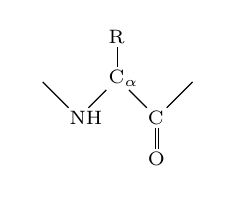
\begin{tikzpicture}
    \tikzstyle{every node}=[inner sep=1, font=\scriptsize, text width=1.5ex]
    % Draw a line at 30 degrees and of length 3
    \node (NH) at (0,0) {NH};
    \node (CA) at ($(NH)+(45:2em)$) {C$_{\alpha}$};
    \node (CO) at ($(CA)+(-45:2em)$) {C};
    \node (O) at ($(CO)+(90:-1.5em)$) {O};
    \node (R) at ($(CA)+(90:1.5em)$) {R};
    \node (DUM0) at ($(NH)+(-45:-2em)$) {};
    \node (DUM1) at ($(CO)+(45:2em)$) {};
    \draw[line width=.1ex] (DUM0) -- (NH) -- (CA) -- (CO) -- (DUM1);
    \draw[line width=.1ex, double] (CO) -- (O);
    \draw[line width=.1ex] (CA) -- (R);
\end{tikzpicture}
\end{document}
